\documentclass{standalone}

\begin{document}

\subsection[Shortcut]{Shortcut connections}\label{NN:shortcut}

The harder becomes the problem to solve and the deeper\footnote{
  The deep of a Neural Network model is related to the number of layers which made it.
} will be the Neural Network model created to solve it.
The payback of these deep Neural Network structures is a reduction in accuracy after reaching a maximum, the so-called \emph{degradation problem}.
This accuracy reduction does not arise from over-fitting problems but it is due to numerical instabilities (\emph{vanishing gradient} - as the gradient is back-propagated to earlier layers, repeated multiplications may make the gradient very small) and troubles related to the data dimensionality (called \emph{curse of dimensionality}).
Despite Neural Network could be defined as universal function approximators, adding numerous layers and thus parameters, the result in accuracy does not grow proportionally.
With simple empirical examples we can easily see how the accuracy starts to saturate (and eventually degrade) with an increasing number of layers.
Those problems pose a limit to the number of layers suitable on a Neural Network model and it seems that the shallower networks learn better than their deeper counterparts.
Keeping this results in mind we can think about a strategy to skip these \quotes{extra} layers.

\begin{center}
\begin{figure}[htbp]
\centering
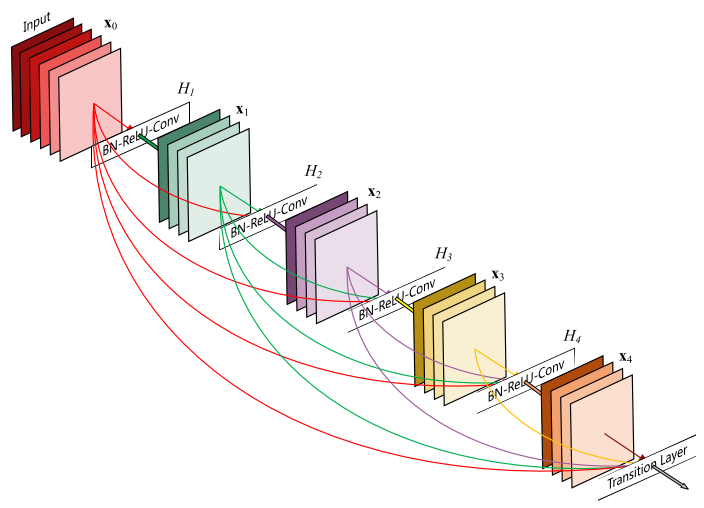
\includegraphics[width=0.85\textwidth]{shortcut_layer.png}
\caption{Scheme of shortcut connections into a deep learning model.
Each colored line connects the previous layer block to the following one.
The output combination can be customized but the most used one is a simple linear combination of them.
A particular attention must be paid with the dimensions management.
}
\label{fig:shortcut}
\end{figure}
\end{center}

We can obtain a simple solution to this issue making extra connections between layers called shortcuts or residuals.
A shortcut is a link between two distant layers without involving the set of layers between them, a so-called \quotes{identity shortcut connection}.
A graphical example is show in Fig.~\ref{fig:shortcut}.
The authors of \cite{he2015deep} argue that stacking layers should not degrade the network performance, because we could simply stack identity mappings (layer that does not do anything) upon the current network, and the resulting architecture would perform the same.
In the original paper, the shortcut connections perform an operation like:

$$
H(x) = F(x_1) + x_2
$$
\\
where $F(x)$ is the output of the previous block and $x$ is the output of the current block.
The function $F$ generalizes the combination of these two values\footnote{
  In our implementations we choose to generalize this formula as

  $$
  H(x) = \alpha x_1 + \beta x_2
  $$
}.

The introduction of these extra connections leads to the ResNet (Residual Neural Network) models era, in which a key role is played by the object detection models.
A wide range of modern deep learning architectures use this kind of connections and in this way they can reach a large number of layers: famous examples of this kind are the VGG models and the ResNets.
We have done a large use of this connections also in the models described in the next sections, either for object detection purposes (ref. \ref{obj_detection:obj}), Super Resolution (ref. \ref{SR:sr}) and mostly in our image segmentation (ref. \ref{segmentation:unet}) application.
This kind of functions are becoming so popular into modern deep learning models that more and more often we describe a model according to its \emph{residual blocks}, i.e the layer ensemble between two shortcut connections.

From a computational point-of-view the implementation of this kind of \quotes{layers} is straightforward in \textsf{Python} (and thus in our \textsf{NumPyNet}): we can easily implement a network structure as a list of objects in which a shortcut connection simply combines the output of two of its elements.
We met more problems when we translated this idea into \textsf{C++}.
The \textsf{C++} language is more rigid with data types involved in each operation and we have to carefully manage the \quotes{signature} (list of input arguments) of each function.
In this way we can not simply implement a list of different object types as a network structure.

A possible solution can be reached using the object inheritance: we can create a single \textsf{Base\_layer} object and specialize it according to our needs.
This is certainly the most \textsf{C++}-like solution but it requires many checks (if statements) at execution time.
An other (more modern) solution is provided by the new (standard) data types provided by the \textsf{C++17}: in particular we refer to the \textsf{variant} objects.
A \textsf{variant} is a \textsf{template union} data type which allows to combine and reinterpret different data types into a single object.
The most important consequence in the usage of this kind of data type is that we can easily jump to one type to an other using \textsf{constexpr} statements which (by definition) are solved at compile time.
Besides the particulars involved into this kind of implementation, it is important to notice that the difference between the two solution is the same between compile-time and run-time, i.e one-for-all against at-every-run.
The \textsf{Byron} library widely use \textsf{template}s and with the support of the \textsf{C++17} standard, a large part of costly operations are execute one-for-all at compile time\footnote{
  We provide also an efficient retro-compatibility for \quotes{old-standard users} with a custom implementation of \textsf{variant} objects.
}.

Using \textsf{variant} objects and \textsf{templates} we can easily implement a shortcut connection also in \textsf{C++} as can be seen on the \href{https://github.com/Nico-Curti/Byron/blob/master/src/shortcut_layer.cpp}{on-line} version of the code.

\end{document}
